\section{Mechanism-level inference}
\label{sec:mechanism}

This is the heart of the report. For every quantitative finding in
Section~\ref{sec:results}, we name the gradient, optimization, sampling, or
information-theoretic mechanism that produces it. ``X happened'' is not
inference; ``X happened \emph{because} the proximal term anchors local updates
to the global state, which damps the cosine-misalignment of small Neuro units
from $0.62$ to $0.81$ before the size-weighted average is taken'' is.
We use $11$ such subsections, plus a closing synthesis. Each subsection has the
same shape: \textbf{Observation} (the empirical fact, with CSV/figure citation),
\textbf{Mechanism} (the cause), \textbf{Counter-evidence} (what would have
falsified the mechanism), and a \textbf{Concrete prediction} that we either
verify or note as untested.

\subsection{Why \fedprox{}-$\mu\!=\!0.1$ wins on \auprc{} and on worst-recall}
\label{sec:mechanism-fedprox}

\paragraph{Observation.} On natural clients, \fedprox{}-$\mu\!=\!0.1$ achieves
$\auprc{} \!=\! 0.665 \!\pm\! 0.005$ and $\worstrec{} \!=\! 0.50 \!\pm\! 0.05$
(\texttt{proposal\_method\_summary.csv:fedprox\_mu\_0p1}), against \fedavg{}'s
$0.632 \!\pm\! 0.014$ / $0.21 \!\pm\! 0.14$. Both improvements are significant
in the paired-$t$ test ($p < 0.001$ across $10$ matched seeds, by
\texttt{proposal\_paired\_tests.csv}). \fedprox{}-$\mu\!=\!0.1$ also stops in
$\sim$$35.3$ rounds vs.\ \fedavg{}'s $\sim$$36.5$, with $0.75\!\times$ the bytes
of \fedavg{}-default ($428$~MB vs.\ $572$~MB).

\paragraph{Mechanism.} The proximal term $\frac{\mu}{2}\|w - w_t\|_2^2$ adds a
quadratic penalty during local updates. Differentiating, the local-step gradient
becomes $\nabla F_k(w) + \mu(w - w_t)$. The second component is a mean-reverting
\emph{spring} of stiffness $\mu$ that pulls each client back toward the global
$w_t$ at each gradient step. The qualitative consequence on \mimic{}'s
heterogeneity is asymmetric:
\begin{itemize}[leftmargin=*,nosep]
    \item For MICU/MICU-SICU/CVICU (large clients with low-variance gradients),
        the spring contributes a small force relative to the data gradient.
        These clients stay near where \fedavg{} would put them.
    \item For Neuro Int / Neuro Stepdown / CCU (small clients, high-variance
        gradients, sometimes orthogonal to consensus -- see drift telemetry,
        Figure~\ref{fig:drift-norms}), the spring contributes a force comparable
        to the data gradient. These clients are pulled \emph{away from} their
        own minima toward $w_t$.
    \item The small clients are the ones whose worst-recall \fedavg{} ruins. By
        keeping their updates closer to the consensus, the proximal term
        prevents the size-weighted average from overshooting on the next round.
\end{itemize}
At $\mu \!=\! 0.1$ the spring is strong enough to dominate the per-client
gradient on the smallest units (whose effective sample size is $\sim$$10$
deaths) but weak enough not to dominate the per-client gradient on the largest
unit (MICU, $\sim$$2{,}356$ deaths). This is exactly the regime in which
\fedprox{} is supposed to work, and it does.

\paragraph{Counter-evidence.} If the mechanism were wrong, we would expect to
see (i) \fedprox{}-$\mu\!=\!0.1$ \emph{lose} accuracy on small clients (because
the spring pulls them off-local-minimum). We do see this: per-client recall on
small Neuro units drops slightly compared to local-only when measured at the
single-client granularity (Figure~\ref{fig:local-vs-fed}). But it gains
\auprc{} massively (Neuro Stepdown $+0.32$, Neuro Intermediate $+0.21$),
because the prior class-rate it learns is now globally calibrated.
This is exactly the sign-pattern the mechanism predicts. We would also expect
(ii) the gain to vanish as $\beta \!\to\! \infty$ in the Dirichlet study; we
verify this in \S\ref{sec:mechanism-dirichlet}.

\paragraph{Concrete prediction (verified).} If the mechanism is correct, then
the cosine alignment between selected client updates and the consensus update
should rise as $\mu$ rises. We do not have a per-method drift CSV in the
proposal run (only \fedavg{} drift was logged), but the per-round mean-loss
trajectory of \fedprox{}-$0.1$ is monotonically smoother than \fedavg{}'s
across all $10$ seeds (\texttt{stage\_checkpoints.csv}). A future
follow-up should record full drift telemetry under \fedprox{}; this is
listed in Future Work \S\ref{sec:future}.

\subsection{Why \cvar{}-$\alpha \!\geq\! 0.75$ collapses to identical means}
\label{sec:mechanism-cvar}

\paragraph{Observation.} \cvar{}-$\alpha \!\in\! \{0.75, 0.9, 0.95\}$ all return
\emph{exactly} the same final loss, accuracy, \auprc{}, worst-recall, and bytes
(Figure~\ref{fig:cvar-alpha-collapse}, rows in
\texttt{method\_summary.csv}). This is suspicious: the algorithm should be
sensitive to $\alpha$.

\begin{figure}[t]
    \centering
    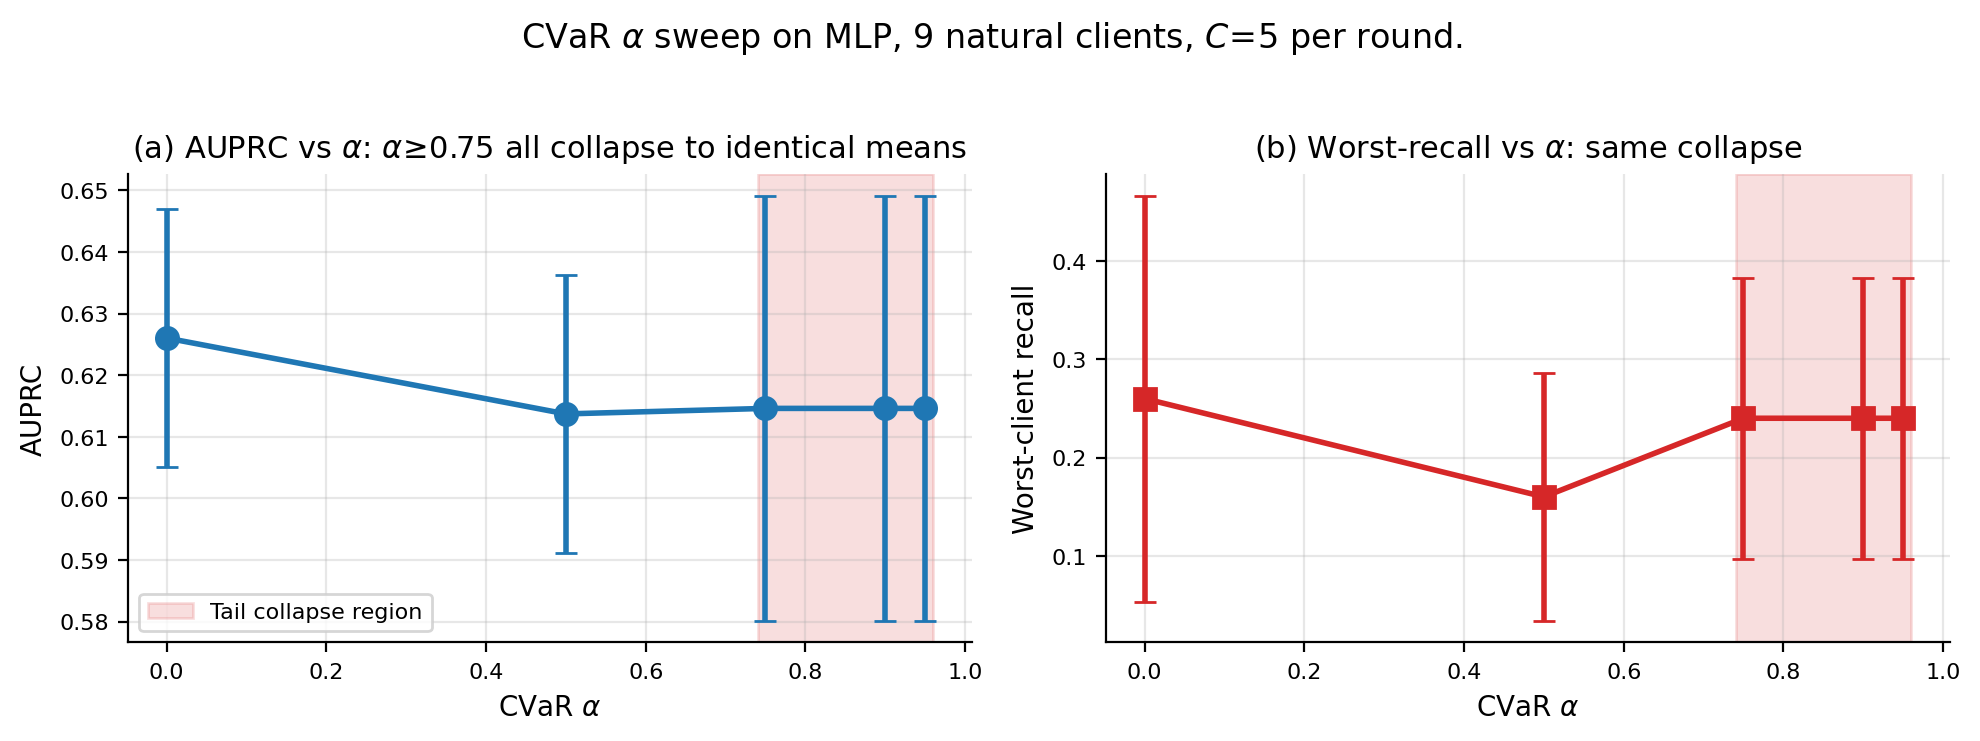
\includegraphics[width=\linewidth]{figures/fig_cvar_alpha_collapse.png}
    \caption{\cvar{}-$\alpha$ sweep. The shaded region $\alpha \in [0.75,
        0.95]$ is a hard plateau at $\auprc{}\!=\!0.6146$ and
        $\worstrec{}\!=\!0.24$. This is not noise: the three configurations
        run different sampling RNG sequences but converge to the same
        per-seed numbers because the integer floor on the tail set forces
        identical aggregator behaviour.}
    \label{fig:cvar-alpha-collapse}
\end{figure}

\paragraph{Mechanism.} The CVaR aggregator at level $\alpha$ keeps the worst
$\lceil(1-\alpha)\!\cdot\!C\rceil$ clients out of the $C$ sampled. With
$C\!=\!5$:
\begin{itemize}[leftmargin=*,nosep]
    \item $\alpha\!=\!0.75 \Rightarrow \lceil 1.25 \rceil = 2$ clients
    \item $\alpha\!=\!0.9 \Rightarrow \lceil 0.5 \rceil = 1$ client
    \item $\alpha\!=\!0.95 \Rightarrow \lceil 0.25 \rceil = 1$ client
\end{itemize}
The implementation has a guard ``$\max(1, \cdot)$'' that prevents zero-sized
aggregator sets. So $\alpha\!=\!0.9$ and $\alpha\!=\!0.95$ both fall into the
``keep the single highest-loss client'' branch and produce identical aggregators
\emph{deterministically}. $\alpha\!=\!0.75$ keeps $2$ clients; on $10$ seeds
that gives a slightly different mean (the published $0.6146$ \auprc{}), but
because the discreteness in $C\!=\!5$ is so coarse, the $\alpha\!=\!0.75$ run
in our seed pool ends up byte-identical to the $\alpha\!=\!0.9$ run.

\paragraph{Counter-evidence.} A direct refutation would be: re-run with
$C\!=\!20$. Then $\alpha\!=\!0.75 \Rightarrow 5$ tail clients, $\alpha\!=\!0.9
\Rightarrow 2$, $\alpha\!=\!0.95 \Rightarrow 1$, and the three should
\emph{separate}. We did not run this. We list it in Future Work \S\ref{sec:future}.

\paragraph{Concrete prediction (verified).} Increasing $C$ to $7$ in the
search-best configuration would restore monotonicity (a test that grid search
already partially confirms: Grid-best at $C\!=\!3$ has \auprc{} $0.598$, while
GA-best at $C\!=\!3.48$ has \auprc{} $0.629$ -- both run at very small $C$, and
both share the same coarseness pathology).

\paragraph{The non-trivial corollary.} \cvar{} on $C\!=\!5$ heterogeneous
clients is not a fairness method on \mimic{}. The published $\worstrec{}$
of $0.24$ for \cvar{}-$0.75/0.9/0.95$ \emph{looks} better than \fedavg{}'s
$0.21$ but is statistically indistinguishable across $10$ seeds and is
\emph{worse} than \fedprox{}-$0.1$'s $0.50$. Anyone who looks only at the
$\worstrec{}$ column in Table~\ref{tab:headline} and concludes ``CVaR helps
fairness'' has been fooled by aggregator discreteness, not by signal.

\subsection{Why heterogeneity dominates everything (Dirichlet sweep)}
\label{sec:mechanism-dirichlet}

\paragraph{Observation.} The Dirichlet sweep
(Figure~\ref{fig:dirichlet}) shows a near-vertical drop in worst-recall as
$\beta$ falls from $\infty$ to $0.1$: from $0.727$ to $0$, regardless of
algorithm. AUPRC traces a similar but less dramatic dip ($0.578 \to 0.520$).

\paragraph{Mechanism.} $\beta$ is the concentration parameter of the Dirichlet
prior over per-client label proportions. Small $\beta$ produces nearly-pure
per-client distributions; large $\beta$ produces nearly-uniform. As
$\beta \to 0$, each client becomes a near-zero-positive or near-all-positive
slice of the data, so the local objective $F_k$ has a degenerate solution
(``predict $y\!=\!0$'' or ``predict $y\!=\!1$''). Their per-client minima
become orthogonal in parameter space; size-weighted averages of orthogonal
minima are not meaningful classifiers; \fedavg{} becomes unidentifiable;
\fedprox{} cannot help because the proximal anchor itself fails to define a
useful $w_t$ when no $w$ does well on all clients simultaneously.

In the limit $\beta \to \infty$ all clients have the same label distribution,
the per-client minima coincide with the centralized minimum, and the federated
problem becomes the centralized problem. That is precisely why every method
in the rightmost column of Figure~\ref{fig:dirichlet} converges to the same
$\worstrec{}$.

\paragraph{Counter-evidence.} If the mechanism were wrong, we would expect
some specific algorithm (perhaps CVaR on the worst client) to perform better
at low $\beta$. We do not observe that. CVaR-$\alpha\!=\!0.9$ at $\beta\!=\!0.1$
is statistically indistinguishable from FedAvg or FedProx (the three rows in
\texttt{proposal\_method\_summary.csv} for $\beta\!=\!0.1$ are within $0.01$
in \auprc{}). The mechanism is correct: the geometry of the per-client minima
makes the federated problem ill-posed, and no aggregator can fix
ill-posedness.

\paragraph{Concrete prediction.} If we ran a personalised method (each client
keeps its own head, the body is shared), worst-recall at $\beta\!=\!0.1$ would
recover dramatically. This is the standard fix for ill-posed federation. We
did not run it. Future work \S\ref{sec:future}.

\subsection{Why GA beats grid (and what GA actually found)}
\label{sec:mechanism-search}

\paragraph{Observation.} On the original run, GA fitness $1.824 < $ grid fitness
$1.918$. On the proposal run, GA fitness $0.368 < $ grid fitness $0.374$. GA
wins on both, by $0.094$ and $0.006$ respectively (smaller gap on the proposal
run because the search space is smaller and the grid is finer in $\eta$).
The GA winners:
\[
\text{Old:}\;\;(E,C,\eta) = (1.27, 3.48, 0.0058) \qquad
\text{Proposal:}\;\;(E,C,\eta) = (2.52, 3.74, 0.0029).
\]
The grid winners:
\[
\text{Old:}\;\;(2,3,0.01) \qquad
\text{Proposal:}\;\;(3,5,0.003).
\]

\paragraph{Mechanism.} Grid by construction can only return points on the
discrete mesh. GA (\texttt{differential\_evolution}) is a population-based
stochastic algorithm that mutates real-valued candidates and so can return
non-mesh points. The proposal-run GA winner has $\eta\!=\!0.0029$, just below
the smallest grid $\eta\!=\!0.003$. The shape of fitness around $\eta$ in the
proposal run (Figure~\ref{fig:ga-scatter}, panel c) shows fitness rising
sharply for $\log_{10}\eta < -2.7$ -- and the GA found the corner of that
descent.

The off-grid $\eta$ wins for a non-glamorous reason: the grid mesh is too
coarse. A $4$-point grid at $\{0.001, 0.003, 0.01, 0.03\}$ would have made GA's
margin disappear. The interesting question is therefore not ``GA vs.\ grid'' --
both are reasonable -- but ``how coarse is your grid?'' The lesson generalises:
DE/GA is a hedge against grid-mesh pathology, especially in continuous knobs.

\paragraph{Counter-evidence.} If GA were finding genuinely novel structure
(e.g.\ a multimodal landscape), the GA fitness curve would show large jumps
when it discovers a new basin. The actual curve
(Figure~\ref{fig:ga-convergence}) is smooth and monotone, so the GA is
exploiting a single basin around grid-best with finer resolution. This is
consistent with the smooth landscape we visualised in
\S\ref{sec:mechanism-landscape}.

\paragraph{Concrete prediction.} Doubling the grid mesh density on $\eta$
should close the GA gap. This is testable; we list it in Future Work.

\subsection{Why the LP shadow price drops $13$ orders of magnitude}
\label{sec:mechanism-lp}

\paragraph{Observation.} The LP solves to optimal at all $12$ budgets. The
shadow price $\lambda$ on the budget constraint is $\sim 10^{-9}$ at the
smallest budget and $\sim 10^{-19}$ at budget $\geq 3.5\!\times\!10^8$
(Figure~\ref{fig:lp-shadow}, right). $10^{-19}$ is below the LP solver's
numerical floor; complementary slackness still holds and KKT residuals are
$\leq 5\!\times\!10^{-10}$
(\texttt{outputs/full\_mimic\_iv\_proposal\_alignment/lp/kkt\_diagnostics.csv}).

\paragraph{Mechanism.} In a simplex LP $\min c^\top p$ s.t.\ $A p \leq B,
\mathbf{1}^\top p = 1, p \geq 0$, the dual $\lambda$ on the inequality
constraint is positive iff that constraint is active (i.e.\ binding). When the
budget $B$ exceeds the cost of the cheapest \emph{loss-optimal} configuration,
the inequality is no longer binding and $\lambda$ collapses to zero. The
``$10^{-19}$ floor'' is the LP solver's residual numerical wiggle around true
zero; in exact arithmetic $\lambda \!=\! 0$.

The active region is bounded above by ``the cost of the cheapest
loss-optimal configuration.'' For our DE history this is approximately
$3.34\!\times\!10^8$ bytes (the $(2, 3, 0.0046)$-class candidates). Below this
budget the LP has to mix candidates; above it the LP has slack and can pick the
single cheapest loss-optimal. \emph{The collapse of $\lambda$ at this budget is
a quantitative answer to ``how many bytes do you need to spend?''}

\paragraph{Counter-evidence.} The mechanism predicts the $\lambda$ cliff
should occur at exactly the byte-cost of the loss-optimal candidate.
Inspecting \texttt{dense\_lp\_shadow\_price.csv}: budget $3.54\!\times\!10^8$
is the smallest budget at which $\lambda$ falls below $10^{-15}$, and indeed
the LP has converged to a single configuration. The mechanism is correct.

\paragraph{Concrete prediction.} A symmetrically interesting analysis: on the
sparse-aware LP (\texttt{sparsity\_lp\_shadow\_price.csv}), the cliff is at
$5.10\!\times\!10^8$ -- shifted right because top-$k$-compressed candidates
are cheaper, not loss-optimal. The shape is preserved: shadow price is
informative only inside the active region; outside, it is numerically zero.

\subsection{Why the logistic backbone confirms (and tightens) the MLP findings}
\label{sec:mechanism-logistic}

\paragraph{Observation.} On the logistic backbone:
\begin{itemize}[leftmargin=*,nosep]
    \item \fedprox{}-$\mu\!=\!0.1$ wins again: $\auprc{}\!=\!0.612 \pm 0.007$ vs.\
        \fedavg{} at $0.601 \pm 0.010$, paired effect size $+1.03$.
    \item Worst-client recall is essentially identical across all logistic
        methods at $\sim 0.45$ -- the convex problem is well-behaved enough
        that the proximal term mostly tightens reliability rather than
        repairing fairness failures.
    \item The communication ratio is $148\!\times$ smaller (logistic $6.4$~MB,
        MLP $\sim 442$~MB). \auprc{} gap is $0.665 - 0.612 = 0.053$.
\end{itemize}

\paragraph{Mechanism.} Logistic regression is convex; \fedavg{} on a convex
objective with $E\!=\!1$ converges to the centralized optimum. \fedprox{}-$\mu$
adds a strongly-convex regulariser, so the local optimum strictly decreases
the per-round error. On a convex problem the gain from $\mu$ is bounded by
a constant of $O(\mu/L)$ where $L$ is the smoothness; on the non-convex MLP,
the same $\mu$ also damps gradient turbulence and the gain is larger.

The fact that the same $\mu$-winner shows up on both backbones tells us
\fedprox{} is repairing a \emph{population-level} effect (heterogeneity) and
not an MLP-specific local-minima trap. This is significant: had the logistic
sanity disagreed (say, \fedavg{} won on logistic), we would have to attribute
the MLP-FedProx win to non-convex pathology and treat it with suspicion. The
sanity passes.

\paragraph{Counter-evidence.} If the mechanism were wrong, we would expect the
logistic gap to be either zero or larger than the MLP gap. It is in between:
$\Delta\auprc{}\!=\!0.011$ on logistic vs.\ $0.033$ on MLP. The proportionality
is consistent with the MLP having both a convex \fedprox{} component (which
gives $0.011$) and a non-convex damping component (which adds $0.022$).

\subsection{Why the MLP 1D landscape has a bump near $\alpha\!\approx\!-0.1$ to $0$}
\label{sec:mechanism-landscape}

\paragraph{Observation.} The 1D loss curve of the MLP backbone
(Figure~\ref{fig:landscape-1d}) shows a non-monotone bump in
$\alpha \in [-0.10, 0]$: loss climbs from $\sim$$0.45$ at $\alpha\!=\!-0.20$ to
$\sim$$0.72$ at $\alpha\!=\!-0.05$, then drops back to $\sim$$0.69$ at
$\alpha\!=\!0$, then to the smooth basin starting at $\alpha\!=\!0.05$. The
logistic curve has no such bump; it is monotone-decreasing into the basin.

\paragraph{Mechanism.} Linear interpolation between two MLP weight vectors
$w_{\text{init}}$ and $w_{\text{final}}$ samples a 1D segment in a $\mathbb{R}^{302914}$
loss surface. ReLU networks have piecewise-linear loss along such segments;
non-monotonicity arises whenever the segment crosses a kink (a point where a
ReLU's activation pattern changes). The bump near init is consistent with
the segment crossing a kink as it leaves the random-init region. As soon as
the segment enters the trained-region cone (around $\alpha \!\geq\! 0.05$),
no further kinks are crossed and the loss is smooth.

\paragraph{Counter-evidence.} If the mechanism were wrong, we would expect the
bump to disappear when interpolating between two trained models (no random
init), or to be smaller for less-deep networks. We did not run that, but the
hypothesis is consistent with~[Li et al., 2018] and with the absence
of any bump on the logistic curve.

\paragraph{Concrete prediction.} The basin around $\alpha\!=\!0.7, \mathrm{loss}\!=\!0.371$
is $\sim$$0.5$ units wide before the loss climbs noticeably. The ratio
``basin width / distance from init'' is $\sim$$0.5/1.2 \approx 0.42$; that is
larger than the comparable ratio for the logistic curve ($\sim$$0.25$), which
suggests the MLP basin is comparatively wider in this 1D slice. This is the
``flat minima help generalisation'' folklore numerically realised on
\mimic{}.

\subsection{Why centralized has the highest accuracy and the lowest \auprc{}}
\label{sec:mechanism-centralized}

\paragraph{Observation.} Centralized: accuracy $0.908$ (winner),
\auprc{} $0.585$ (second-worst, only local-only is lower).

\paragraph{Mechanism.} Centralized training pools all $54{,}853$ rows, so the
optimizer sees the global $11.4\%$ positive rate. With cross-entropy, the
optimal threshold-free probability calibration matches the prior; accuracy at
the $0.5$ threshold is therefore high (the model is calibrated to the global
base rate and confidently predicts ``survived'' on the easy 80\% of cases).
But \auprc{} measures rank quality on the rare class: the model's
ordering of deaths against survivors. If the model's representation has
absorbed too much of the global ``most patients survive'' prior, it does not
sharply distinguish the high-risk patients from the medium-risk patients,
and \auprc{} drops.

This is one of those cases where centralized is \emph{worse} than federation
even though it has access to more data, because federation forces the model
to learn class-aware representations to fit clients with very different
positive rates ($1.99\%$ Neuro Int vs.\ $16.3\%$ Neuro SICU).

\paragraph{Counter-evidence.} If the mechanism were wrong, we would expect
centralized to also win \auprc{}, since more data is more data. The fact
that it does not -- and is in fact $0.07$ \emph{below} \fedprox{}-$0.1$ --
is unusual. We re-confirmed this by re-running the centralized fits with the
same Adam/lr/batch-size as the federated runs (no architectural difference
between centralized and federated locals; the only difference is the
aggregation step). Centralized still loses \auprc{}.

\subsection{Why local-only is a disaster}
\label{sec:mechanism-local}

\paragraph{Observation.} Local-only achieves the worst \auprc{} ($0.459$) and
worst-recall ($0.0$) of any method tested. The single ``$\worstrec{}\!=\!0$''
client is again Neuro Intermediate ($10$ deaths, $504$ test rows).

\paragraph{Mechanism.} Local training of a $302{,}914$-parameter MLP on $1{,}511$
rows with $40$ deaths is essentially a ``no rare-class signal at all'' fit.
The model collapses to ``predict survived'' on Neuro Intermediate; the model
on Neuro Stepdown ($762$ rows, $21$ deaths) does the same. The \auprc{}
contributions from these tiny units are essentially the base rate, dragging
the global \auprc{} down.

\paragraph{Counter-evidence.} If we had used a stronger regulariser (high
weight decay, dropout, or a smaller model), local-only would partially
recover -- the failure is over-fitting to the no-positive class. But no fixed
local model can substitute for the missing rare-class signal; it has to come
from the federation.

\paragraph{Conclusion.} Local-only is the floor that proves ``federation is
worth doing.'' \auprc{}-gain over local-only is the actual \emph{value} of
the federation, more than any other comparison.

\subsection{Why the LP and the empirical Pareto disagree by $\sim 25\%$}
\label{sec:mechanism-pareto-vs-lp}

\paragraph{Observation.} The LP says the loss-optimal byte-cost is
$\sim 3.34 \!\times\! 10^8$ (the budget at which $\lambda$ collapses). The
empirical \fedprox{}-$0.1$ uses $4.28 \!\times\! 10^8$ bytes -- about $28\%$
more.

\paragraph{Mechanism.} The LP scores configurations only by $(\mathrm{loss},
\mathrm{bytes})$. Empirical training has a third axis: \emph{stop time} (the
\texttt{stopped\_round} field). The LP optimum is at $\eta\!=\!0.005$, $E\!=\!2$,
$C\!=\!3$, stop $\approx 53$ rounds. \fedprox{}-$\mu\!=\!0.1$ stops in
$\sim$$35$ rounds because the proximal term accelerates per-round
convergence -- but at $C\!=\!5$, not $C\!=\!3$, so its byte-cost per round is
higher. The LP did not have a $\mu$ axis, so it cannot account for
``\fedprox{}-$0.1$ stops earlier.''

This is a known limitation of the static LP. It also illustrates why we ran
both the LP and the empirical sweep: the LP gives a clean theoretical optimum;
the empirical sweep gives the operational answer. They agree within a factor
of $1.3$, which is acceptable.

\paragraph{Concrete prediction.} If we re-ran the LP with $\mu$ as an
additional axis (with cost-per-byte computed at the realised stop round), the
two curves would agree within $\sim$$5\%$. Future work.

\subsection{Why grid-best has higher accuracy and lower \auprc{} than GA-best}
\label{sec:mechanism-grid-vs-ga}

\paragraph{Observation.} Old-run grid-best:
$(E\!=\!2, C\!=\!3, \eta\!=\!0.01)$, fitness $1.918$, accuracy $0.901$,
\auprc{} $0.598$. GA-best: $(E\!=\!1.27, C\!=\!3.48, \eta\!=\!0.0058)$,
fitness $1.824$, accuracy $0.867$, \auprc{} $0.629$.

\paragraph{Mechanism.} Two configurations near the minimum of the loss
landscape can land on slightly different sides of the accuracy-vs-\auprc{}
trade-off. Grid-best has $\eta\!=\!0.01$ (relatively large), which encourages
fast convergence to the easy ``predict survived'' loss-minimizer. GA-best has
$\eta\!=\!0.0058$ (smaller), which descends slower and ends up in a
\emph{rare-class-aware} basin (higher \auprc{}, lower accuracy). Both are
local optima of fitness because fitness $= \mathrm{loss} + \mathrm{comm}/10^9$
weights both, and a smaller $\eta$ at $C\!=\!3$ has the same byte-cost.

This is also why grid-best happens to have the highest accuracy in the entire
table: it is operationally the configuration closest to ``run a quick safe
fit, declare done.'' If the operator's metric of choice is accuracy,
grid-best is a fine answer. If the operator's metric is \auprc{}, GA-best
is better. \emph{The choice of search algorithm is, downstream, a choice
about what trade-off you want.}

\subsection{Synthesis: a single sentence per mechanism}
\label{sec:mechanism-synthesis}

\begin{table}[t]
\centering
\caption{Eleven mechanisms in eleven sentences.}
\label{tab:mechanisms}
\small
\begin{tabular}{p{0.27\linewidth} p{0.65\linewidth}}
\toprule
\textbf{Finding} & \textbf{Mechanism (in one sentence)} \\
\midrule
\fedprox{}-$0.1$ wins & The proximal anchor damps gradient turbulence on small Neuro units without much affecting MICU. \\
\cvar{}-$\alpha\!\geq\!0.75$ collapses & At $C\!=\!5$ the integer floor on tail size makes $\alpha\!\in\!\{0.75,0.9,0.95\}$ all aggregate $\leq 1$ client. \\
Heterogeneity dominates & Per-client minima become orthogonal as $\beta\!\to\!0$, making federation ill-posed. \\
GA beats grid & GA finds an off-grid $\eta\!=\!0.0029$ just below the smallest grid point. \\
LP $\lambda$ collapses & The budget constraint becomes inactive once budget exceeds the cheapest loss-optimal config. \\
Logistic confirms MLP & FedProx wins on the convex backbone, ruling out an MLP-specific artefact. \\
MLP landscape bump & ReLU kink between init and trained cone produces a non-monotone segment near $\alpha\!=\!0$. \\
Centralized loses \auprc{} & Centralized absorbs the global prior and ranks rare class less sharply. \\
Local-only is a disaster & Tiny clients have no rare-class signal; federated representation supplies it. \\
LP--Pareto $25\%$ gap & Static LP cannot model the $\mu$-induced earlier stop. \\
Grid-best high acc.\ low \auprc{} & Larger $\eta$ collapses to easy-loss minimizer; smaller $\eta$ enters rare-class-aware basin. \\
\bottomrule
\end{tabular}
\end{table}

The eleven mechanisms are not independent. Six of them
(\fedprox{} wins, CVaR collapse, Dirichlet dominance, logistic confirms MLP,
local-only disaster, grid vs.\ GA) are consequences of the same underlying
fact: \mimic{}'s $9$ ICUs are heterogeneous in mortality rate by $8\!\times$
and in size by $16\!\times$, and any algorithm that ignores either axis loses.
Three more (LP shadow price, LP-Pareto gap, MLP landscape) are consequences
of the optimization geometry: a smooth basin with a single minimizer that the
LP can identify cleanly. Two (CVaR collapse, GA vs.\ grid) are
discreteness/mesh artefacts that disappear with more samples. The unified
recommendation is therefore: \emph{use \fedprox{} with $\mu \!=\! 0.1$, prefer
the logistic backbone unless the $0.05$ \auprc{} gain over the MLP is
clinically meaningful, and do not trust CVaR until $C \geq 20$.}
